\documentclass[a4paper,oneside,DIV=12,12pt,headings=normal]{scrartcl}

%%% Length calculations
\usepackage{calc}
%%%

%%% Support for color
\usepackage{xcolor}
\definecolor{lightblue}{HTML}{03A9F4}
\definecolor{red}{HTML}{F44336}
%%%

%%% Graphics inclusion
\usepackage{graphicx}
%%%

%%% Font selection
\usepackage{fontspec}

\setromanfont{STIX Two Text}[
	SmallCapsFeatures = {LetterSpace = 5},
]

\setsansfont{Source Sans Pro}[
]

\setmonofont{Source Code Pro}[
]
%%%

%%% Math settings
\usepackage{amsmath,unicode-math}
\setmathfont{STIX Two Math}

% \usepackage{IEEEtrantools}
\usepackage{mleftright}
%%%

%%% Font settings for different KOMA Script elements
\setkomafont{pagenumber}{\rmfamily}
\setkomafont{disposition}{\rmfamily\bfseries}
%%%

%%% Typographic enhancements
\usepackage{microtype}
%%%

%%% Language-specific settings
\usepackage{polyglossia}
\setmainlanguage{ukrainian}
%%%

%%% List settings
\usepackage{enumitem}
\setlist[enumerate]{
	leftmargin = *,
}
%%%

%%% Captions
\usepackage{caption}
\usepackage{subcaption}

\DeclareCaptionLabelFormat{closing}{#2)}
\captionsetup[subtable]{labelformat = closing}
\captionsetup[subfigure]{labelformat = closing, position = auto}
%%%

%%% Tables
\usepackage{booktabs}
\usepackage{longtable}

\usepackage{multirow}

\usepackage{array}
\newcolumntype{v}[1]{>{\raggedright\arraybackslash\hspace{0pt}}p{#1}}
\newcolumntype{b}[1]{>{\centering\arraybackslash\hspace{0pt}}p{#1}}
\newcolumntype{n}[1]{>{\raggedleft\arraybackslash\hspace{0pt}}p{#1}}

\usepackage{kbordermatrix} % labeling array indices
%%%

%%% Floats on a single row
\usepackage{floatrow}
\newfloatcommand{capbtabbox}{table}[][\FBwidth]
%%%

%%% Links and hyperreferences
\usepackage{hyperref}
\hypersetup{
	colorlinks      = false,
	linkbordercolor = red,
	urlbordercolor  = lightblue,
	pdfborderstyle  = {/S/U/W 1.5},
}
%%%

%%% All caps
\newcommand{\allcaps}[1]{{\addfontfeatures{LetterSpace = 3}#1}}
%%%

\setlength{\emergencystretch}{1em}

\begin{document}
	\hyphenation{муль-ти-плек-со-рів де-муль-ти-плек-со-рів}
	\begin{titlepage}
	\centering
		Міністерство освіти і науки України\\
		Національний авіаційний університет\\
		Навчально-науковий інститут комп'ютерних інформаційних технологій\\
		Кафедра комп'ютеризованих систем управління

		\vspace*{\fill}

		Лабораторна робота №2\\
		з дисципліни «Комп'ютерна схемотехніка»\\
		на тему «Дослідження мультиплексорів і демультиплексорів»

		\vspace*{\fill}
		
		\begin{flushright}
			Виконав:\\
			студент ННІКІТ СП-225\\
			Клокун В.\,Д.\\
			Перевірив:\\
			Іскренко Ю.\,Ю.
		\end{flushright}

		Київ 2018
    \end{titlepage}
	
	\section{Мета роботи}
		Вивчення логіки роботи, принципів побудови й синтезу мультиплексорів і демультиплексорів, а також методики дослідження схем мультиплексорів і демультиплексорів. Визначення основних характеристик і параметрів мультиплексорів і~демультиплексорів на інтегральних мікросхемах. Ознайомлення з мікросхемами мультиплексорів і демультиплексорів вітчизняних серій \allcaps{ТТЛШ}, \allcaps{ЕЗЛ} і~\allcaps{КМОН}.
		
	\section{Хід роботи}
		\subsection{Дослідження схеми мультиплексора «2—1»}
			Складаємо схему мультиплексора на два інформаційних входи~$X_0$, $X_1$, один інформаційний вихід~$D$ і один адресний вхід~$A_0$~(рис.~\ref{fig:01-mul-2-1-schematic}). За результатами експерименту заповнюємо таблицю істинності~(табл.~\ref{tab:01-mul-2-1-truthtable}).
			
			\begin{figure}[!htbp]
				\begin{floatrow}
					\ffigbox[\Xhsize/2]{
						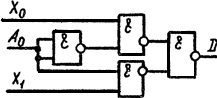
\includegraphics[]{./assets/01.png}
					}{
						\caption{Схема мультиплексора «2—1»}
						\label{fig:01-mul-2-1-schematic}
					}
					\capbtabbox[\Xhsize]{
						\begin{tabular}{*{3}{l}r}
							\toprule
								$A_0$ & $X_1$ & $X_0$ & $D$ \\
							\midrule
								0     & 0     & 0     & 0\\
								0     & 0     & 1     & 1\\
								0     & 1     & 0     & 0\\
								0     & 1     & 1     & 1\\
								1     & 0     & 0     & 0\\
								1     & 0     & 1     & 0\\
								1     & 1     & 0     & 1\\
								1     & 1     & 1     & 1\\
							\bottomrule
						\end{tabular}
					}{
						\caption{Таблиця істинності мультиплексора «2—1»}
						\label{tab:01-mul-2-1-truthtable}
					}
				\end{floatrow}
			\end{figure}
			
		\subsection{Дослідження схеми мультиплексора «4—1»}
			Складаємо схему мультиплексора на чотири інформаційних входи~$X_0, \dots, X_3$, один інформаційних вихід~$D$, і два адресних входи~$A_0$, $A_1$~(рис.~\ref{fig:02-mul-4-1-schematic}). За результатами експерименту заповнюємо таблицю істинності~(табл.~\ref{tab:02-mul-4-1-truthtable}).
			
			\begin{figure}[!htbp]
				\begin{floatrow}
					\ffigbox[\Xhsize/2]{
						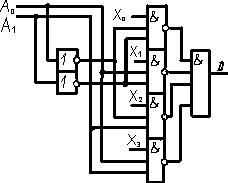
\includegraphics[height = 10\baselineskip]{./assets/02.png}
					}{
						\caption{Схема мультиплексора «4—1»}
						\label{fig:02-mul-4-1-schematic}
					}
					\capbtabbox[\Xhsize]{
						\begin{tabular}{*{6}{l}r}
							\toprule
								$A_1$ & $A_0$ & $X_3$ & $X_2$ & $X_1$ & $X_0$ & $D$ \\
							\midrule
								0     & 0     & 0     & 0     & 0     & 0     & 0\\
								0     & 0     & 0     & 0     & 0     & 1     & 1\\
								0     & 1     & 0     & 0     & 0     & 0     & 0\\
								0     & 1     & 0     & 0     & 1     & 0     & 1\\
								1     & 0     & 0     & 0     & 0     & 0     & 0\\
								1     & 0     & 0     & 1     & 0     & 0     & 1\\
								1     & 1     & 0     & 0     & 0     & 0     & 0\\
								1     & 1     & 1     & 0     & 0     & 0     & 1\\
							\bottomrule
						\end{tabular}
					}{
						\caption{Таблиця істинності мультиплексора «4—1»}
						\label{tab:02-mul-4-1-truthtable}
					}
				\end{floatrow}
			\end{figure}
			
		\subsection{Дослідження схеми мультиплексора «4—1» у режимі реалізації логічних функцій}
			За допомогою мультиплексора «4—1»~(рис.~\ref{fig:02-mul-4-1-schematic}) будуємо таблицю істинності заданої у~\allcaps{ДДНФ} функції~$F = \neg A_1 \land \neg A_0 \lor A_1 \land A_0$.
			
			\begin{table}[!htbp]
			\centering
				\begin{tabular}{*{2}{l}r}
					\toprule
						$A_1$ & $A_0$ & $F = D$ \\
					\midrule
						0     & 0     & 1\\
						0     & 1     & 0\\
						1     & 0     & 0\\
						1     & 1     & 1\\
					\bottomrule
				\end{tabular}
			\caption{Таблиця істинності заданої функції}
			\label{tab:03-logicalfunction}
			\end{table}
			
		\subsection{Дослідження схеми демультиплексора «1—2»}
			Складаємо схему демультиплексора на один інформаційних вхід~$D$, два інформаційних виходи~$X_0$, $X_1$ і один адресний вхід~$A_0$~(рис.~\ref{fig:04-demul-1-2-schematic}). За результатами експерименту заповнюємо таблицю істинності~(табл.~\ref{tab:04-demul-1-2-truthtable}).
			
			\begin{figure}[!htbp]
				\begin{floatrow}
					\ffigbox[\Xhsize/2]{
						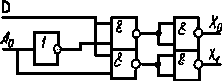
\includegraphics[height = 5\baselineskip]{./assets/03.png}
					}{
						\caption{Схема демультиплексора «1—2»}
						\label{fig:04-demul-1-2-schematic}
					}
					\capbtabbox[\Xhsize]{
						\begin{tabular}{*{2}{l}*{2}{r}}
							\toprule
								$A_0$ & $D$ & $X_1$ & $X_2$ \\
							\midrule
								0     & 0   & 0     & 0 \\
								0     & 1   & 0     & 1\\
								1     & 0   & 1     & 0\\
								1     & 1   & 1     & 1\\
							\bottomrule
						\end{tabular}
					}{
						\caption{Таблиця істинності демультиплексора «1—2»}
						\label{tab:04-demul-1-2-truthtable}
					}
				\end{floatrow}
			\end{figure}
			
		\subsection{Дослідження схеми демультиплексора «1—4»}
			Складаємо схему демультиплексора на один інформаційних вхід~$D$, чотири інформаційних виходи~$X_0, \dots, X_3$ і два адресних входи~$A_0$~(рис.~\ref{fig:05-demul-1-4-schematic}). За результатами експерименту заповнюємо таблицю істинності~(табл.~\ref{tab:05-demul-1-4-truthtable}).
			
			\begin{figure}[!htbp]
				\begin{floatrow}
					\ffigbox[\Xhsize/2]{
						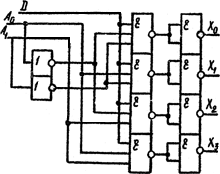
\includegraphics[height = 10\baselineskip]{./assets/04.png}
					}{
						\caption{Схема демультиплексора «1—4»}
						\label{fig:05-demul-1-4-schematic}
					}
					\capbtabbox[\Xhsize]{
						\begin{tabular}{*{3}{l}*{4}{r}}
							\toprule
								$A_1$ & $A_0$ & $D$ & $X_3$ & $X_2$ & $X_1$ & $X_0$ \\
							\midrule
								0     & 0     & 0   & 0     & 0     & 0     & 0\\
								0     & 0     & 1   & 0     & 0     & 0     & 1\\
								0     & 1     & 0   & 0     & 0     & 0     & 0\\
								0     & 1     & 1   & 0     & 0     & 1     & 0\\
								1     & 0     & 0   & 0     & 0     & 0     & 0\\
								1     & 0     & 1   & 0     & 1     & 0     & 0\\
								1     & 1     & 0   & 0     & 0     & 0     & 0\\
								1     & 1     & 1   & 1     & 0     & 0     & 0\\
							\bottomrule
						\end{tabular}
					}{
						\caption{Таблиця істинності демультиплексора «1—4»}
						\label{tab:05-demul-1-4-truthtable}
					}
				\end{floatrow}
			\end{figure}
			
	\section{Висновок}
		Під час виконання даної лабораторної роботи ми вивчили логіку роботи, принципи побудови й синтезу мультиплексорів і демультиплексорів. Освоїли методики дослідження схем мультиплексорів і демультиплексорів. Визначили основних характеристик і параметрів мультиплексорів і демультиплексорів на інтегральних мікросхемах. Ознайомились з мікросхемами мультиплексорів і демультиплексорів вітчизняних серій \allcaps{ТТЛШ}, \allcaps{ЕЗЛ} і~\allcaps{КМОН}.
		
\end{document}
